\input templates/header

\usepackage[normalem]{ulem}
\usepackage{xcolor}
\usepackage{tikz}
\usetikzlibrary{trees}
\usetikzlibrary{shapes}
\usetikzlibrary{positioning}


\usepackage{xmpmulti}
\usepackage{listings}


\newcommand{\FCNB}{
  \begin{tabular}{c|c}
    \multicolumn{2}{c}{} \\\hline
    \, & \, 
  \end{tabular}
}

\newcommand{\FA}{
  \begin{tabular}{c|c|c|c}
    \multicolumn{4}{c}{\emph{P}} \\\hline
    \, & \, & \, & \,
  \end{tabular}
}    
\newcommand{\FB}{
  \begin{tabular}{c|c|c|c}
    \multicolumn{4}{c}{\emph{P}} \\\hline
    . & \, & \, & \,
  \end{tabular}  
}    
\newcommand{\FC}{
  \begin{tabular}{c|c|c|c}
    \multicolumn{4}{c}{\emph{P}} \\\hline
    . & . & \, & \,
  \end{tabular}
}    
\newcommand{\FD}{
  \begin{tabular}{c|c|c|c}
    \multicolumn{4}{c}{\emph{P}} \\\hline
    . & . & . & \,
  \end{tabular}
}    


% \newcommand*{\ml}[2][c]{\tabular[t]{@{}#1@{}} #2 \endtabular}
% \makeatletter
% \newcommand*{\Strut}[1][1em]{\vrule\@width\z@\@height#1\@Depth\z@\relax}
% \makeatother

\lstset{
  basicstyle=\ttfamily,
  columns=fullflexible,
  keywordstyle=\color{red}\bfseries,
  commentstyle=\color{blue},
  showstringspaces=false,
	escapeinside={(*@}{@*)},
}


\definecolor{ocra}{rgb}{1.0,0.9,0.7}
\definecolor{azzurro}{rgb}{0.8,0.8,1.0}

\title[ASD - Strutture dati]{\textbf{Algoritmi e Strutture Dati}\\[24pt]
Alberi}

\graphicspath{{figs/05/}}

\begin{document}






%-------------------------------------------------------------------------
\FrameTitle{}

%-------------------------------------------------------------------------
\FrameContent

%%%%%%%%%%%%%%%%%%%%%%%%%%%%%%%%%%%%%%%%%%%%%%%%%%%%%%%%%%%%%%%%%%%%%%%%%%
\section{Introduzione}
%%%%%%%%%%%%%%%%%%%%%%%%%%%%%%%%%%%%%%%%%%%%%%%%%%%%%%%%%%%%%%%%%%%%%%%%%%

%%%%%%%%%%%%%%%%%%%%%%%%%%%%%%%%%%%%%%%%%%%%%%%%%%%%%%%%%%%%%%%%%%%%%%%%%%
\subsection{Esempi}
%%%%%%%%%%%%%%%%%%%%%%%%%%%%%%%%%%%%%%%%%%%%%%%%%%%%%%%%%%%%%%%%%%%%%%%%%%


%-------------------------------------------------------------------------
%----------------------------------------------------------------------
\begin{frame}{Esempio 1}

\IG{0.6}{biology.png}

\end{frame}

%-------------------------------------------------------------------------
%----------------------------------------------------------------------
\begin{frame}{Esempio 2}


\IG{1.0}{directory.png}

\end{frame}

%-------------------------------------------------------------------------
%----------------------------------------------------------------------
\begin{frame}[fragile,shrink=5]{Esempio 3}

\vspace{-12pt}
\begin{lstlisting}[language=html,tabsize=2]
<html>
    <head>
        <meta http-equiv="Content-Type" content="text/html"/>
        <title>simple</title>
    </head>
    <body>
        <h1>A simple web page</h1>
        <ul>
            <li>List item one</li>
            <li>List item two</li>
        </ul>
        <h2>
            <a href="http://www.google.com">Google</a>
        </h2>
    </body>
</html>
\end{lstlisting}

\end{frame}

%-------------------------------------------------------------------------
%----------------------------------------------------------------------
\begin{frame}{Esempio 3}

\begin{center}
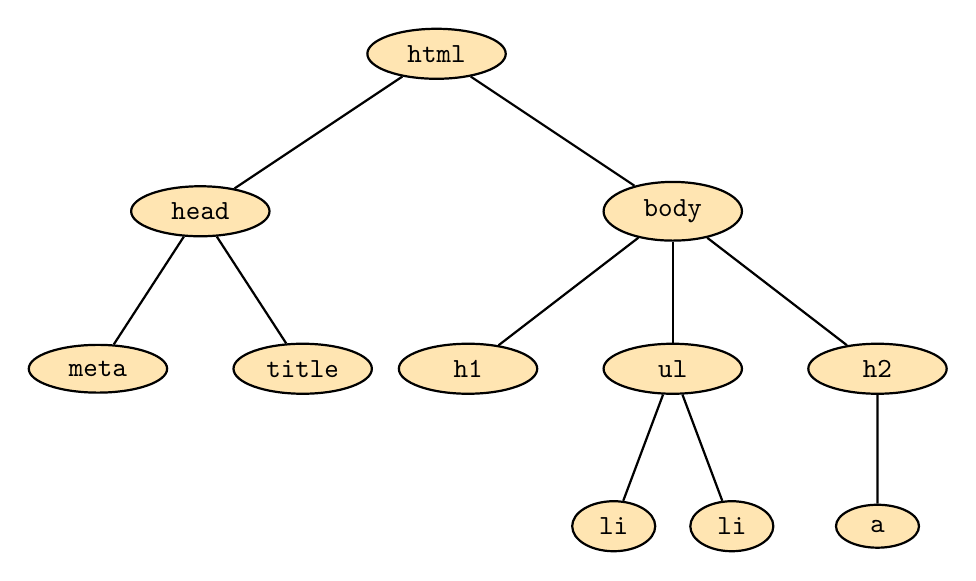
\begin{tikzpicture}[
	level distance=2cm,
  level 1/.style={sibling distance=6cm},
  level 2/.style={sibling distance=2.6cm},
  level 3/.style={sibling distance=1.5cm},
	thick,
	font=\ttfamily\bfseries]
	\tikzstyle{every node}=[thick,draw, ellipse, minimum width=50pt,align=center,fill=ocra]
  \node {html}
    child {node {head}
      child {node {meta}}
      child {node {title}}
    }
    child {node {body}
      child {node {h1}}
      child {node {ul}
		child {node[minimum width=30pt] {li}}
		child {node[minimum width=30pt] {li}}
	  }
      child {node {h2}
		child {node[minimum width=30pt] {a}
      }
	}
  };
\end{tikzpicture}
\end{center}


\end{frame}



%%%%%%%%%%%%%%%%%%%%%%%%%%%%%%%%%%%%%%%%%%%%%%%%%%%%%%%%%%%%%%%%%%%%%%%%%%
\subsection{Definizioni}
%%%%%%%%%%%%%%%%%%%%%%%%%%%%%%%%%%%%%%%%%%%%%%%%%%%%%%%%%%%%%%%%%%%%%%%%%%

%-------------------------------------------------------------------------
%----------------------------------------------------------------------
\begin{frame}{Albero radicato -- Definizione 1}

\begin{myboxtitle}[Albero radicato (Rooted tree)]
Un albero consiste di un insieme di nodi e un insieme di archi orientati che connettono coppie di nodi, con le seguenti proprietà:
\BIL
\item Un nodo dell'albero è designato come nodo \alert{radice};
\item Ogni nodo $n$, a parte la radice, ha esattamente un arco
entrante;
\item Esiste un cammino unico dalla radice ad ogni nodo;
\item L'albero è connesso.
\EIL
\end{myboxtitle}
\end{frame}

%-------------------------------------------------------------------------
%----------------------------------------------------------------------
\begin{frame}[fragile]{Albero radicato -- Definizione 2 (Ricorsiva)}

\begin{myboxtitle}[Albero radicato (Rooted tree)]
Un albero è dato da:
\BI
\item un insieme vuoto, oppure
\item un nodo \alert{radice} e zero o più \alert{sottoalberi}, ognuno dei quali è un albero; la radice è connessa alla radice di ogni sottoalbero con un arco orientato.
\EI
\end{myboxtitle}

\begin{center}
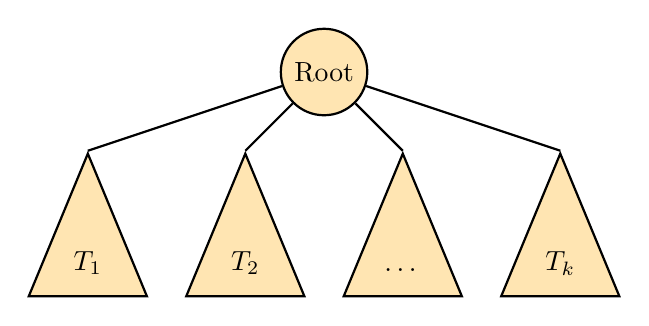
\begin{tikzpicture}[level/.style={sibling distance = 2cm/#1,level distance = 1cm},thick]
\tikzset{
    treenode/.style = {circle, draw=black, align=center, minimum size=1cm,fill=ocra},
    subtree/.style  = {isosceles triangle, draw=black, align=center, minimum height=1.5cm, minimum width=1.5cm, shape border rotate=90, anchor=north, fill=ocra}
}	
\node [treenode] {Root}
   child [child anchor=north]
   {
      node [subtree] {$T_1$} 
   }
	 child [child anchor=north]
	 {
	 node [subtree] {$T_2$} 
	 }
	 child [child anchor=north]
	 {
	 node [subtree] {\ldots} 
	 }
	 child [child anchor=north]
	 {
	 node [subtree] {$T_k$} 
	 }
;
\end{tikzpicture}
\end{center}

\end{frame}

%-------------------------------------------------------------------------
%----------------------------------------------------------------------
\begin{frame}{Terminologia}

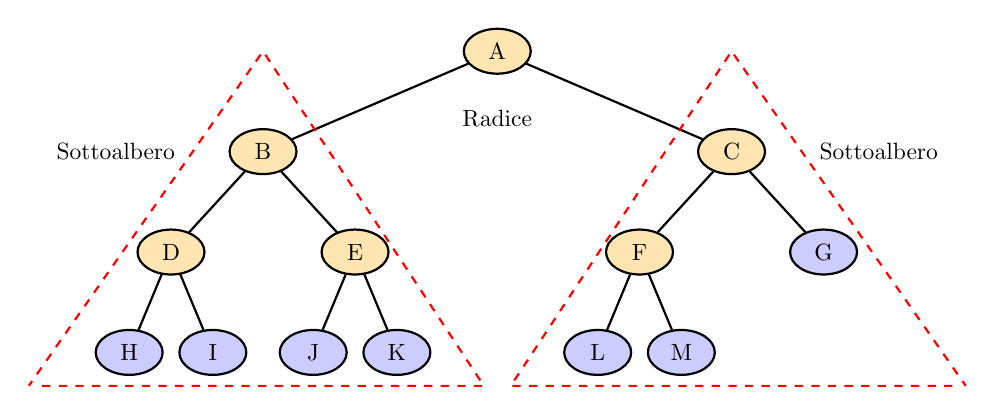
\begin{tikzpicture}[
	scale=0.85, 
	transform shape,
	level distance=1.5cm,
  level 1/.style={sibling distance=7cm},
  level 2/.style={sibling distance=2.75cm},
  level 3/.style={sibling distance=1.25cm},
	thick
]
\tikzset{
    treenode/.style = {ellipse, draw=black, align=center,fill=ocra,minimum width=1cm, minimum height=0.5cm},
    subtree/.style  = {isosceles triangle, draw=black, align=center, minimum height=3cm, minimum width=6cm, shape border rotate=90, dashed}
}
\node (root) [treenode] {A}
  child { node[treenode] (B) {B} 
  	child { node[treenode] {D} 
			child { node[treenode,fill=azzurro] {H} }
  		child { node[treenode,fill=azzurro] {I} }
		}
  	child { node[treenode] {E} 
			child { node[treenode,fill=azzurro] {J} }
  		child { node[treenode,fill=azzurro] {K} }
		}
	}
  child { node[treenode] {C} 
  	child { node[treenode] {F}	
			child { node[treenode,fill=azzurro] {L} }
  		child { node[treenode,fill=azzurro] {M} }
		}
  	child { node[treenode,fill=azzurro] {G} }
	}
;	
\node at (-5.7,-1.5) {\alert{Sottoalbero}};
\node at (5.7,-1.5) {\alert{Sottoalbero}};
\node [below of=root] {\alert{Radice}};
\draw [dashed,red] (-6.8,-5) -- (-0.2,-5)  -- (-3.5, 0) -- (-7,-5);
\draw [dashed,red] (6.8,-5) -- (0.2,-5)  -- (3.5, 0) -- (7,-5);

\end{tikzpicture}

\begin{multicols}{3}
\BI
\item $A$ è la \alert{radice}
\item $B,C$ sono radici dei sottoalberi
\item $D,E$ sono \alert{fratelli}
\columnbreak
\item $D,E$ sono \alert{figli} di $B$
\item $B$ è il \alert{padre} di $D,E$
\columnbreak
\item I nodi viola sono \alert{foglie}
\item Gli altri nodi sono \alert{nodi interni}
\EI
\end{multicols}
\end{frame}




%-------------------------------------------------------------------------
%----------------------------------------------------------------------
\begin{frame}{Terminology (English)}

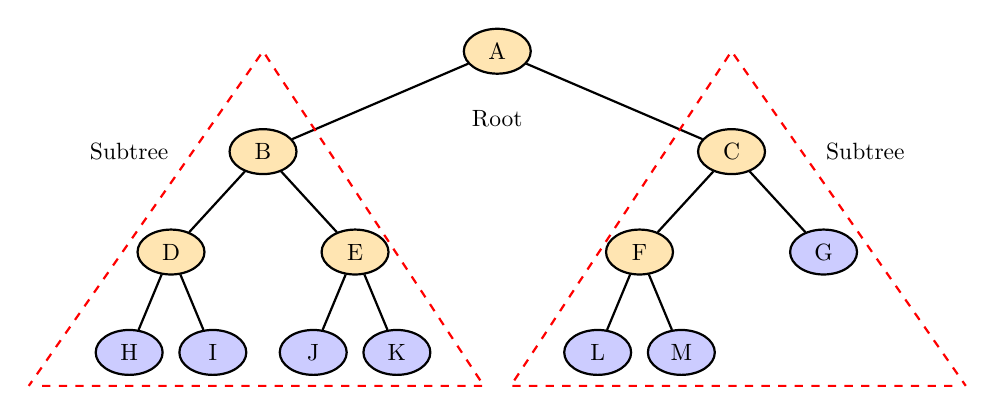
\begin{tikzpicture}[
	scale=0.85, 
	transform shape,
	level distance=1.5cm,
  level 1/.style={sibling distance=7cm},
  level 2/.style={sibling distance=2.75cm},
  level 3/.style={sibling distance=1.25cm},
	thick
]
\tikzset{
    treenode/.style = {ellipse, draw=black, align=center,fill=ocra,minimum width=1cm, minimum height=0.5cm},
    subtree/.style  = {isosceles triangle, draw=black, align=center, minimum height=3cm, minimum width=6cm, shape border rotate=90, dashed}
}
\node (root) [treenode] {A}
  child { node[treenode] (B) {B} 
  	child { node[treenode] {D} 
			child { node[treenode,fill=azzurro] {H} }
  		child { node[treenode,fill=azzurro] {I} }
		}
  	child { node[treenode] {E} 
			child { node[treenode,fill=azzurro] {J} }
  		child { node[treenode,fill=azzurro] {K} }
		}
	}
  child { node[treenode] {C} 
  	child { node[treenode] {F}	
			child { node[treenode,fill=azzurro] {L} }
  		child { node[treenode,fill=azzurro] {M} }
		}
  	child { node[treenode,fill=azzurro] {G} }
	}
;	
\node at (-5.5,-1.5) {\alert{Subtree}};
\node at (5.5,-1.5) {\alert{Subtree}};
\node [below of=root] {\alert{Root}};
\draw [dashed,red] (-6.8,-5) -- (-0.2,-5)  -- (-3.5, 0) -- (-7,-5);
\draw [dashed,red] (6.8,-5) -- (0.2,-5)  -- (3.5, 0) -- (7,-5);

\end{tikzpicture}

\begin{multicols}{3}
\BI
\item $A$ is the tree \alert{root}
\item $B,C$ are roots of their subtrees
\item $D,E$ are \alert{siblings}
\item $D,E$ are \alert{children} of $B$
\item $B$ is the \alert{parent} of $D,E$
\item Purple nodes are \alert{leaves}
\item The other nodes are \alert{internal nodes}
\EI
\end{multicols}
\end{frame}

%-------------------------------------------------------------------------
%----------------------------------------------------------------------
\begin{frame}{Terminologia}
\vspace{-12pt}

\TwoCols{
\begin{myboxtitle}[Profondità nodi (Depth)]
La lunghezza del cammino semplice dalla radice al nodo
(misurato in numero di archi)
\end{myboxtitle}
\begin{myboxtitle}[Livello (Level)]
L'insieme di nodi alla stessa profondità
\end{myboxtitle}
\begin{myboxtitle}[Altezza albero (Height)]
La profondità massima della sue foglie
\end{myboxtitle}
}{
\smallskip
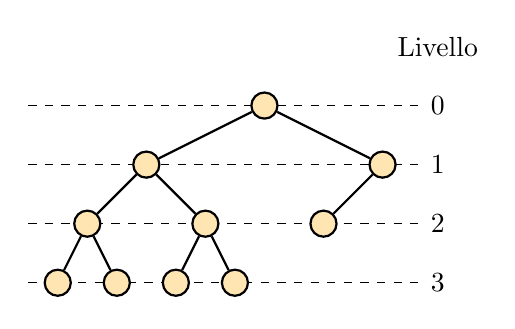
\begin{tikzpicture}[
	level distance=0.75cm,
  level 1/.style={sibling distance=3cm},
  level 2/.style={sibling distance=1.5cm},
  level 3/.style={sibling distance=0.75cm},
	thick
]
\tikzset{
    treenode/.style = {circle, draw=black, align=center,fill=ocra},
}	
\draw[dashed,thin] (-3,0) -- (2,0);
\draw[dashed,thin] (-3,-0.75) -- (2,-0.75);
\draw[dashed,thin] (-3,-1.5) -- (2,-1.5);
\draw[dashed,thin] (-3,-2.25) -- (2,-2.25);
\node at (2.2, 0.75) {Livello};
\node at (2.2, 0) {0};
\node at (2.2, -0.75) {1};
\node at (2.2, -1.5) {2};
\node at (2.2, -2.25) {3};

\node (A) [treenode] {}
  child { node[treenode] {} 
  	child { node[treenode] {} 
			child { node[treenode] {} }
  		child { node[treenode] {} }
		}
  	child { node[treenode] {} 
			child { node[treenode] {} }
  		child { node[treenode] {} }
		}
	}
  child { node[treenode] {} 
  	child { node[treenode] {}	}
  	child[missing] { node[treenode] {} }
	}
;

\end{tikzpicture}

\bigskip
\begin{center}
Altezza di questo albero = 3
\end{center}
}

\end{frame}


%%%%%%%%%%%%%%%%%%%%%%%%%%%%%%%%%%%%%%%%%%%%%%%%%%%%%%%%%%%%%%%%%%%%%%%%%%
\section{Alberi binari}
%%%%%%%%%%%%%%%%%%%%%%%%%%%%%%%%%%%%%%%%%%%%%%%%%%%%%%%%%%%%%%%%%%%%%%%%%%

%%%%%%%%%%%%%%%%%%%%%%%%%%%%%%%%%%%%%%%%%%%%%%%%%%%%%%%%%%%%%%%%%%%%%%%%%%
\subsection{Introduzione}
%%%%%%%%%%%%%%%%%%%%%%%%%%%%%%%%%%%%%%%%%%%%%%%%%%%%%%%%%%%%%%%%%%%%%%%%%%

%-------------------------------------------------------------------------
%----------------------------------------------------------------------
\begin{frame}{Albero binario}
	
\vspace{-12pt}
\begin{myboxtitle}[Albero binario]
Un \alert{albero binario} è un albero radicato in cui ogni nodo ha 
al massimo due figli, identificati come figlio \alert{sinistro} e figlio \alert{destro}.
\end{myboxtitle}

\smallskip
\textbf{\alert{Nota}}: \emph{Due alberi $T$ e $U$ che hanno gli stessi nodi, 
gli stessi figli per ogni nodo e la stessa radice, sono distinti qualora un nodo 
$u$ sia designato come figlio sinistro di $v$ in $T$ e come figlio destro 
di $v$ in $U$.}

\begin{center}
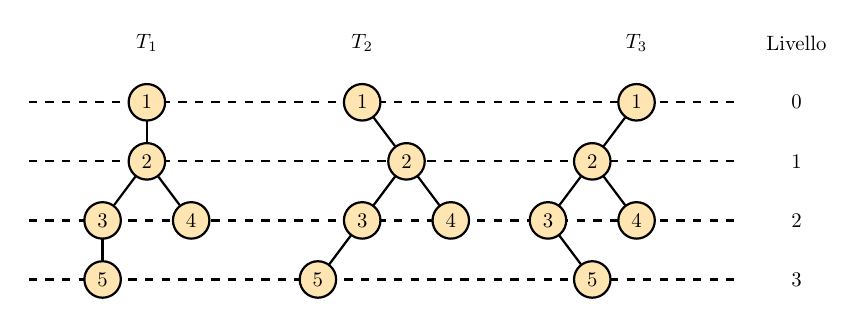
\begin{tikzpicture}[
	thick,
	scale=0.75, 
	transform shape,
	level distance=1cm,
  each level/.style={sibling distance=1cm}
]
\tikzset{
    treenode/.style = {circle, draw=black, align=center,fill=ocra},
}	

\draw[dashed] (-2,0) -- (10,0);
\draw[dashed] (-2,-1) -- (10,-1);
\draw[dashed] (-2,-2) -- (10,-2);
\draw[dashed] (-2,-3) -- (10,-3);

\node (A) [treenode] {1}
child { node[treenode] {2} 
  child { node[treenode] {3} 
		child {node[treenode] {5}} 
	}
  child { node[treenode] {4} }
}
;
\node[above of=A] {$T_1$};
\node (B) [treenode, right=3cm of A] {1}
child[missing] {node {}}
child { node[treenode](B2) {2} 
  child { node[treenode] {3} 
		child {node[treenode] {5}} 
		child[missing] {node {}}
	}
  child { node[treenode] {4} }
}
;
\node[above of=B] {$T_2$};
\node (C) [treenode, right=4cm of B] {1}
child  { node[treenode] (C2) {2} 
  child { node[treenode] {3} 
		child[missing] {node {}}
		child {node[treenode] {5}} 
	}
  child { node[treenode] {4} }
}
child[missing] {node {}}
;
\node[above of=C] {$T_3$};
\node at (11, 1) {Livello};
\node at (11, 0) {0};
\node at (11, -1) {1};
\node at (11, -2) {2};
\node at (11, -3) {3};
\end{tikzpicture}
\end{center}

\end{frame}

%-------------------------------------------------------------------------
%----------------------------------------------------------------------
\begin{frame}{Specifica (Albero binario)}

\begin{Procedure}
\caption[A]{\Tree}

\% Costruisce un nuovo nodo, contenente $v$, senza figli o genitori \;
\alert{$\treeconstructor(\Item\ v)$}\;
\BlankLine

\% Legge il valore memorizzato nel nodo \;
\alert{$\Item\ \treeread()$}\;
\BlankLine

\% Modifica il valore memorizzato nel nodo \;
\alert{$\treewrite(\Item\ v)$}\;
\BlankLine

\% Restituisce il padre, oppure \Nil se questo nodo è radice\;
\alert{$\Tree\ \treeparent()$}\;
\BlankLine

\end{Procedure}

\end{frame}

%-------------------------------------------------------------------------
%----------------------------------------------------------------------
\begin{frame}{Specifica (Albero binario)}

\begin{Procedure}
\caption[A]{\Tree}

\% Restituisce il figlio sinistro (destro) di questo nodo; restituisce \Nil se assente\;
\alert{\Tree\ \treeleft()}\;
\alert{\Tree\ \treeright()}\;
\BlankLine

\% Inserisce il sottoalbero radicato in $t$ come figlio sinistro (destro) di questo nodo\;
\alert{\insertleft(\Tree $t$)}\;
\alert{\insertright(\Tree $t$)}\;
\BlankLine

\% Distrugge (ricorsivamente) il figlio sinistro (destro) di questo nodo \;
\alert{\deleteleft()}\;
\alert{\deleteright()}\;
\BlankLine

\end{Procedure}


\end{frame}

\subsection{Implementazione}

%----------------------------------------------------------------------
\begin{frame}{Memorizzare un albero binario}
	
\vspace{-12pt}
\begin{center}
\includegraphics{albero-bin-store.pdf}
\end{center}

\begin{myboxtitle}[Campi memorizzati nei nodi]
\BI
\item \alert{$\Parentvar$}: reference al nodo padre
\item \alert{$\Leftvar$}: reference al figlio sinistro
\item \alert{$\Rightvar$}: reference al figlio destro
\EI
\end{myboxtitle}

\end{frame}


%----------------------------------------------------------------------
\begin{frame}[shrink=15]{Implementazione}

\vspace{-12pt}
\TwoCols{
\begin{Procedure}
\caption[A]{\Tree}

\PROCEDURE{\alert{\treeconstructor(\Item $v$)}}
{
  $\Tree\ t = \NEW\ \Tree$\;
  $t.\Parentvar = \Nil$\;
  $t.\Leftvar = t.\Rightvar = \Nil$\;
  $t.\Valuevar = v$\;
  \Return $t$\;
}
\BlankLine

\PROCEDURE{\alert{\insertleft(\Tree $T$)}}
{
  \If{$\Leftvar \Eq \Nil$}{
	  $T.\Parentvar = \THIS$\;
  	  $\Leftvar = T$\;
	}
}
\BlankLine

\PROCEDURE{\alert{\insertright(\Tree $T$)}}
{
  \If{$\Rightvar \Eq \Nil$}{
  	$T.\Parentvar = \THIS$\;
  	$\Rightvar = T$\;
	}
}
\end{Procedure}
}{
\includegraphics[width=1.0\linewidth]{albero-bin-store.pdf}
}


\end{frame}

%----------------------------------------------------------------------
\begin{frame}[shrink=15]{Implementazione}

\vspace{-12pt}
\TwoCols{
\begin{Procedure}
\caption[A]{\Tree}


\PROCEDURE{\alert{\deleteleft()}}
{
  \If{$\Leftvar \neq \Nil$}
  {
    $\Leftvar.\deleteleft()$\;
    $\Leftvar.\deleteright()$\;
	\DELETE $\Leftvar$\;
    $\Leftvar = \Nil$\;
  }
}
\BlankLine

\PROCEDURE{\alert{\deleteright()}}
{
  \If{$\Rightvar \neq \Nil$}
  {
    $\Rightvar.\deleteleft()$\;
    $\Rightvar.\deleteright()$\;
	\DELETE $\Rightvar$\;
    $\Rightvar = \Nil$\;
  }
}
\end{Procedure}
}{
\includegraphics[width=1.0\linewidth]{albero-bin-store.pdf}
}

\end{frame}

% \begin{frame}[fragile,shrink=5]{Python}
%
% \vspace{-12pt}
% \begin{multicols}{2}
% \begin{lstlisting}[language=python]
% class BinaryTree:
%   def __init__(self,item):
%     self.value = item
%     self.parent = None
%     self.left = None
%     self.right = None
%
%   def insertLeft(self,tree):
%     if self.left == None:
%       tree.parent = self
%       self.left = tree
%
%   def insertRight(self,tree):
%     if self.right == None:
%       tree.parent = self
%       self.right = tree
%
%   def getRight(self):
%     return self.right
%
%   def getLeft(self):
%     return self.left
%
%   def getValue(self):
%     return self.value
%
%   def setValue(self,item):
%     self.value = item
%
% # To be completed....
% \end{lstlisting}
% ~\\
% ~\\
% \end{multicols}
% \end{frame}


\subsection{Visite}

%----------------------------------------------------------------------
\begin{frame}{Visite di alberi}

\vspace{-3pt}
\begin{myboxtitle}[Visita di un albero  / ricerca]
Una strategia per analizzare (visitare) tutti i nodi di un albero. 
\end{myboxtitle}

\vspace{-3pt}
\TwoCols{
\BB{\alert{Visità in profondità\\ Depth-First Search (DFS)}}
\BIL
\item Per visitare un albero, si visita ricorsivamente ognuno dei suoi \alert{sottoalberi}
\item Tre varianti: pre/in/post visita (\alert{pre/in/post order})
\item Richiede uno \alert{stack}
\EIL
}{
\BB{\alert{Visita in ampiezza\\ Breadth First Search (BFS)}}
\BI
\item Ogni \alert{livello} dell'albero viene visitato, uno dopo l'altro
\item Si parte dalla radice
\item Richiede una \alert{queue}
\EI
}
\end{frame}

%----------------------------------------------------------------------
\begin{frame}{Depth-First Search}
	
\vspace{-12pt}
\TwoCols{
\begin{Procedure}
\caption[A]{\textsf{dfs}(\Tree $t$)}
\If{$t \neq \Nil$}
  {
    \% pre-order visit of $t$\;
		\PRINT $t$\;
		\BlankLine
    $\textsf{dfs}(t.\treeleft())$\;
		\BlankLine
    \% in-order visit of $t$\;
		\PRINT $t$\;
		\BlankLine
    $\textsf{dfs}(t.\treeright())$\;
		\BlankLine
    \% post-order visit of $t$\;
		\PRINT $t$\;
  }
\end{Procedure}
}{
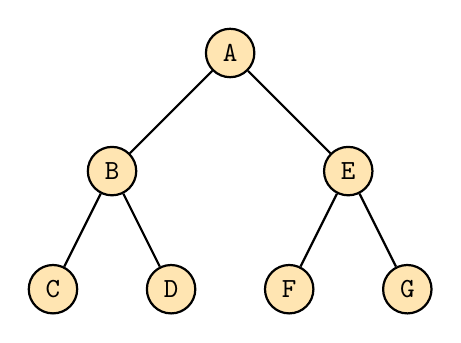
\begin{tikzpicture}[
	thick,
	level distance=1.5cm,
  level 1/.style={sibling distance=3cm},
  level 2/.style={sibling distance=1.5cm},
	font=\ttfamily\bfseries]
  \node[circle,draw,fill=ocra] {A}
    child {node[circle,draw,fill=ocra] {B}
      child {node[circle,draw,fill=ocra] {C}}
      child {node[circle,draw,fill=ocra] {D}}
    }
    child {node[circle,draw,fill=ocra] {E}
    child {node[circle,draw,fill=ocra] {F}}
      child {node[circle,draw,fill=ocra] {G}}
    };
\end{tikzpicture}
}

\end{frame}

%----------------------------------------------------------------------
\begin{frame}{Depth-First Search - Pre-Order}
	
\vspace{-12pt}
\TwoCols{
\begin{Procedure}
\caption[A]{\textsf{dfs}(\Tree $t$)}
\If{$t \neq \Nil$}
  {
    \alert{\% pre-order visit of $t$}\;
		\alert{\PRINT $t$}\;
		\BlankLine
    $\textsf{dfs}(t.\treeleft())$\;
		\BlankLine
    \sout{\% in-order visit of $t$}\;
		\sout{\PRINT $t$}\;
		\BlankLine
    $\textsf{dfs}(t.\treeright())$\;
		\BlankLine
    \sout{\% post-order visit of $t$}\;
		\sout{\PRINT $t$}\;
  }
\end{Procedure}
}{
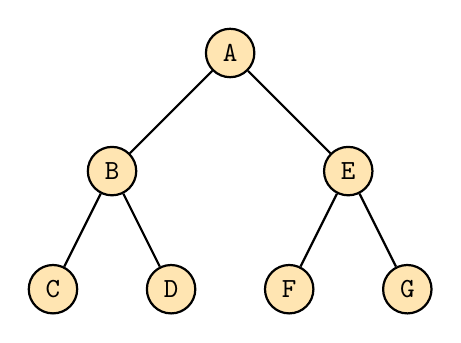
\begin{tikzpicture}[level distance=1.5cm,
	thick,
  level 1/.style={sibling distance=3cm},
  level 2/.style={sibling distance=1.5cm},
	font=\ttfamily\bfseries]
  \node[circle,draw,fill=ocra] {A}
    child {node[circle,draw,fill=ocra] {B}
      child {node[circle,draw,fill=ocra] {C}}
      child {node[circle,draw,fill=ocra] {D}}
    }
    child {node[circle,draw,fill=ocra] {E}
    child {node[circle,draw,fill=ocra] {F}}
      child {node[circle,draw,fill=ocra] {G}}
    };

\end{tikzpicture}

\bigskip
\begin{overprint}
\onslide<1|handout:0>
Sequence: \alert{\texttt{A}}\\
Stack: \alert{\texttt{A}}
\onslide<2|handout:0>
Sequence: \alert{\texttt{A  B}}\\
Stack: \alert{\texttt{A  B}}
\onslide<3|handout:0>
Sequence: \alert{\texttt{A  B  C}}\\
Stack: \alert{\texttt{A  B  C}}
\onslide<4|handout:0>
Sequence: \alert{\texttt{A  B  C}}\\
Stack: \alert{\texttt{A  B}}
\onslide<5|handout:0>
Sequence: \alert{\texttt{A  B  C  D}}\\
Stack: \alert{\texttt{A  B  D}}
\onslide<6|handout:0>
Sequence: \alert{\texttt{A  B  C  D}}\\
Stack: \alert{\texttt{A  B}}
\onslide<7|handout:0>
Sequence: \alert{\texttt{A  B  C  D}}\\
Stack: \alert{\texttt{A}}
\onslide<8|handout:0>
Sequence: \alert{\texttt{A  B  C  D  E}}\\
Stack: \alert{\texttt{A  E}}
\onslide<9|handout:0>
Sequence: \alert{\texttt{A  B  C  D  E  F}}\\
Stack: \alert{\texttt{A  E  F}}
\onslide<10|handout:0>
Sequence: \alert{\texttt{A  B  C  D  E  F}}\\
Stack: \alert{\texttt{A  E}}
\onslide<11|handout:0>
Sequence: \alert{\texttt{A  B  C  D  E  F  G}}\\
Stack: \alert{\texttt{A  E  G}}
\onslide<12|handout:0>
Sequence: \alert{\texttt{A  B  C  D  E  F  G}}\\
Stack: \alert{\texttt{A  E}}
\onslide<13|handout:0>
Sequence: \alert{\texttt{A  B  C  D  E  F  G}}\\
Stack: \alert{\texttt{A}}
\onslide<14|handout:1>
Sequence: \alert{\texttt{A  B  C  D  E  F  G}}\\
Stack: 
\end{overprint}
}
\end{frame}


%----------------------------------------------------------------------
\begin{frame}{Depth-First Search - In-Order}
	
\TwoCols{
\vspace{-12pt}
\begin{Procedure}
\caption[A]{\textsf{dfs}(\Tree $t$)}
\If{$t \neq \Nil$}
  {
    \sout{\% pre-order visit of $t$}\;
		\sout{\PRINT $t$}\;
		\BlankLine
    $\textsf{dfs}(t.\treeleft())$\;
		\BlankLine
    \alert{\% in-order visit of $t$}\;
		\alert{\PRINT $t$}\;
		\BlankLine
    $\textsf{dfs}(t.\treeright())$\;
		\BlankLine
    \sout{\% post-order visit of $t$}\;
		\sout{\PRINT $t$}\;
  }
\end{Procedure}
}{
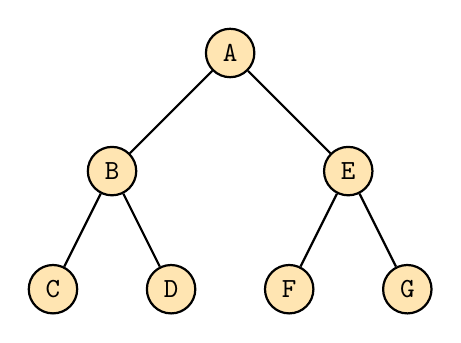
\begin{tikzpicture}[level distance=1.5cm,
	thick,
	level distance=1.5cm,
  level 1/.style={sibling distance=3cm},
  level 2/.style={sibling distance=1.5cm},
	font=\ttfamily\bfseries]
  \node[circle,draw,fill=ocra] {A}
    child {node[circle,draw,fill=ocra] {B}
      child {node[circle,draw,fill=ocra] {C}}
      child {node[circle,draw,fill=ocra] {D}}
    }
    child {node[circle,draw,fill=ocra] {E}
    child {node[circle,draw,fill=ocra] {F}}
      child {node[circle,draw,fill=ocra] {G}}
    };

\end{tikzpicture}

\bigskip
\begin{overprint}
\onslide<1|handout:0>
Sequence: \\
Stack: \alert{\texttt{A}}
\onslide<2|handout:0>
Sequence: \\
Stack: \alert{\texttt{A  B}}
\onslide<3|handout:0>
Sequence: \alert{\texttt{C}}\\
Stack: \alert{\texttt{A  B  C}}
\onslide<4|handout:0>
Sequence: \alert{\texttt{C  B}}\\
Stack: \alert{\texttt{A  B}}
\onslide<5|handout:0>
Sequence: \alert{\texttt{C  B  D}}\\
Stack: \alert{\texttt{A  B  D}}
\onslide<6|handout:0>
Sequence: \alert{\texttt{C  B  D}}\\
Stack: \alert{\texttt{A  B}}
\onslide<7|handout:0>
Sequence: \alert{\texttt{C  B  D  A}}\\
Stack: \alert{\texttt{A}}
\onslide<8|handout:0>
Sequence: \alert{\texttt{C  B  D  A}}\\
Stack: \alert{\texttt{A  E}}
\onslide<9|handout:0>
Sequence: \alert{\texttt{C  B  D  A  F}}\\
Stack: \alert{\texttt{A  E  F}}
\onslide<10|handout:0>
Sequence: \alert{\texttt{C  B  D  A  F  E}}\\
Stack: \alert{\texttt{A  E}}
\onslide<11|handout:0>
Sequence: \alert{\texttt{C  B  D  A  F  E  G}}\\
Stack: \alert{\texttt{A  E  G}}
\onslide<12|handout:0>
Sequence: \alert{\texttt{C  B  D  A  F  E  G}}\\
Stack: \alert{\texttt{A  E}}
\onslide<13|handout:0>
Sequence: \alert{\texttt{C  B  D  A  F  E  G}}\\
Stack: \alert{\texttt{A}}
\onslide<14|handout:1>
Sequence: \alert{\texttt{C  B  D  A  F  E  G}}\\
Stack: 
\end{overprint}
}
\end{frame}


%----------------------------------------------------------------------
\begin{frame}{Depth-First Search - Post-Order}
	
\TwoCols{
\vspace{-12pt}
\begin{Procedure}
\caption[A]{\textsf{dfs}(\Tree $t$)}
\If{$t \neq \Nil$}
  {
    \sout{\% pre-order visit of $t$}\;
		\sout{\PRINT $t$}\;
		\BlankLine
    $\textsf{dfs}(t.\treeleft())$\;
		\BlankLine
    \sout{\% in-order visit of $t$}\;
		\sout{\PRINT $t$}\;
		\BlankLine
    $\textsf{dfs}(t.\treeright())$\;
		\BlankLine
    \alert{\% post-order visit of $t$}\;
		\alert{\PRINT $t$}\;
  }
\end{Procedure}
}{
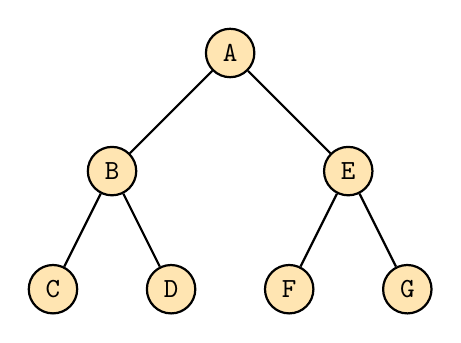
\begin{tikzpicture}[level distance=1.5cm,
	level distance=1.5cm,
  level 1/.style={sibling distance=3cm},
  level 2/.style={sibling distance=1.5cm},
	thick,
	font=\ttfamily\bfseries]
  \node[circle,draw,fill=ocra] {A}
    child {node[circle,draw,fill=ocra] {B}
      child {node[circle,draw,fill=ocra] {C}}
      child {node[circle,draw,fill=ocra] {D}}
    }
    child {node[circle,draw,fill=ocra] {E}
    child {node[circle,draw,fill=ocra] {F}}
      child {node[circle,draw,fill=ocra] {G}}
    };

\end{tikzpicture}

\bigskip
\begin{overprint}
\onslide<1|handout:0>
Sequence: \\
Stack: \alert{\texttt{A}}
\onslide<2|handout:0>
Sequence: \\
Stack: \alert{\texttt{A  B}}
\onslide<3|handout:0>
Sequence: \alert{\texttt{C}}\\
Stack: \alert{\texttt{A  B  C}}
\onslide<4|handout:0>
Sequence: \alert{\texttt{C}}\\
Stack: \alert{\texttt{A  B}}
\onslide<5|handout:0>
Sequence: \alert{\texttt{C  D}}\\
Stack: \alert{\texttt{A  B  D}}
\onslide<6|handout:0>
Sequence: \alert{\texttt{C  D  B}}\\
Stack: \alert{\texttt{A  B}}
\onslide<7|handout:0>
Sequence: \alert{\texttt{C  D  B}}\\
Stack: \alert{\texttt{A}}
\onslide<8|handout:0>
Sequence: \alert{\texttt{C  D  B}}\\
Stack: \alert{\texttt{A  E}}
\onslide<9|handout:0>
Sequence: \alert{\texttt{C  D  B  F}}\\
Stack: \alert{\texttt{A  E  F}}
\onslide<10|handout:0>
Sequence: \alert{\texttt{C  D  B  F}}\\
Stack: \alert{\texttt{A  E}}
\onslide<11|handout:0>
Sequence: \alert{\texttt{C  D  B  F  G}}\\
Stack: \alert{\texttt{A  E  G}}
\onslide<12|handout:0>
Sequence: \alert{\texttt{C  D  B  F  G  E}}\\
Stack: \alert{\texttt{A  E}}
\onslide<13|handout:0>
Sequence: \alert{\texttt{C  D  B  F  G  E  A}}\\
Stack: \alert{\texttt{A}}
\onslide<14|handout:1>
Sequence: \alert{\texttt{C  D  B  F  G  E  A}}\\
Stack: 
\end{overprint}
}
\end{frame}




%----------------------------------------------------------------------
\begin{frame}{Esempi di applicazione}

\BB{Contare nodi -- Post-visita}
\TwoCols{
\begin{Procedure}
\caption[A]{$\INTEGER\ \textsf{count}(\Tree\ T)$}
\eIf{$T \Eq \Nil$}{
  \Return $0$\;
}{
	$C_\ell = \textsf{count}(T.\treeleft())$\;
	$C_r = \textsf{count}(T.\treeright())$\;
	\Return $C_\ell+C_r+1$\;
}
\end{Procedure}
}{
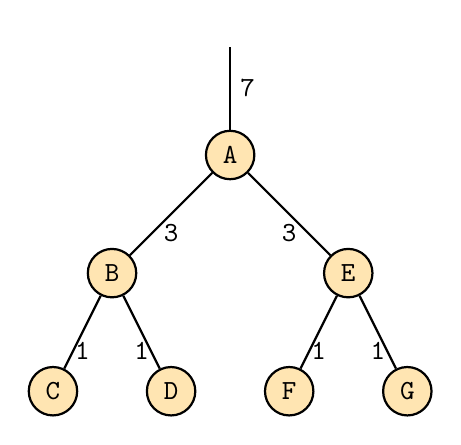
\begin{tikzpicture}[level distance=1.5cm,
	thick,
	level distance=1.5cm,
  level 2/.style={sibling distance=3cm},
  level 3/.style={sibling distance=1.5cm},
	font=\ttfamily\bfseries]
  \node[missing] {}
		child {node[circle,draw,fill=ocra] {A}
    	child {node[circle,draw,fill=ocra] {B}  
      	child {node[circle,draw,fill=ocra] {C} edge from parent node[right,below,draw=none] {1}}
      	child {node[circle,draw,fill=ocra] {D} edge from parent node[left,below,draw=none] {1}}
				edge from parent node[right,below,draw=none] {3}
    	}
    	child {node[circle,draw,fill=ocra] {E} 
      	child {node[circle,draw,fill=ocra] {F} edge from parent node[right,below,draw=none] {1}}
      	child {node[circle,draw,fill=ocra] {G} edge from parent node[left,below,draw=none] {1}}
				edge from parent node[left,below,draw=none] {3}
    	}
			edge from parent node[right,draw=none] {7}
	  };
\end{tikzpicture}
}
\end{frame}

%----------------------------------------------------------------------
\begin{frame}{Esempi di applicazione}

\BB{Stampare espressioni -- In-visita}
\vspace{-12pt}
\TwoCols{
\begin{Procedure}
\caption[A]{$\INTEGER\ \textsf{printExp}(\Tree\ T)$}
\eIf{$T.\treeleft() \Eq \Nil$ \AND $T.\treeright \Eq \Nil$}{
	\PRINT $T.\treeread()$\;
}{
	\PRINT "(" \;
	$\textsf{printExp}(T.\treeleft())$\;
	\PRINT $T.\treeread()$\;
	$\textsf{printExp}(T.\treeright())$\;
	\PRINT ")" \;
}
\end{Procedure}
}{
\begin{center}
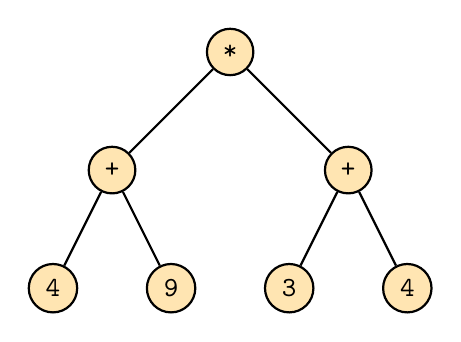
\begin{tikzpicture}[
	level distance=1.5cm,
  level 1/.style={sibling distance=3cm},
  level 2/.style={sibling distance=1.5cm},
	thick,
	font=\ttfamily\bfseries]
  \node[circle,draw,fill=ocra] {*}
    	child {node[circle,draw,fill=ocra] {+}  
      	child {node[circle,draw,fill=ocra] {4}}
      	child {node[circle,draw,fill=ocra] {9}}
    	}
    	child {node[circle,draw,fill=ocra] {\texttt{+}} 
      	child {node[circle,draw,fill=ocra] {3}}
      	child {node[circle,draw,fill=ocra] {4}}
    	}
;
\end{tikzpicture}

\bigskip
\texttt{((4+9) * (3+4))}
\end{center}
}
\end{frame}

%----------------------------------------------------------------------
\begin{frame}{Costo computazionale}

\BB{
Il costo di una visita di un albero contenente $n$ nodi è $\Theta(n)$, in quanto ogni nodo viene visitato al massimo una volta.
}

\end{frame}


\section{Alberi generici}

\vspace{-12pt}
%----------------------------------------------------------------------
\begin{frame}{Specifica (Albero generico)}

\begin{Procedure}
\caption[A]{\Tree}

\% Costruisce un nuovo nodo, contenente $v$, senza figli o genitori \;
\alert{$\treeconstructor(\Item\ v)$}\;
\BlankLine

\% Legge il valore memorizzato nel nodo \;
\alert{$\Item\ \treeread()$}\;
\BlankLine

\% Modifica il valore memorizzato nel nodo \;
\alert{$\treewrite(\Item\ v)$}\;
\BlankLine

\% Restituisce il padre, oppure \Nil se questo nodo è radice\;
\alert{$\Tree\ \treeparent()$}\;
\BlankLine

\end{Procedure}

\end{frame}

%----------------------------------------------------------------------
\begin{frame}{Specifica (Albero generico)}

\vspace{-12pt}
\begin{Procedure}
\caption[A]{\Tree}

\% Restituisce il primo figlio, oppure \Nil se questo nodo è una foglia\;
\alert{$\Tree\ \treechild()$}\;

\% Restituisce il prossimo fratello, oppure \Nil se assente\;
\alert{$\Tree\ \treesibling()$}\;
\BlankLine

\% Inserisce il sottoalbero $t$ come primo figlio di questo nodo\;
\alert{$\insertchild(\Tree\ t)$}\;
\BlankLine

\% Inserisce il sottoalbero $t$ come prossimo fratello di questo nodo\;
\alert{$\insertsibling(\Tree\ t)$}\;
\BlankLine

\% Distruggi l'albero radicato identificato dal primo figlio \;
\alert{$\deletechild()$}\;
\BlankLine

\% Distruggi l'albero radicato identificato dal prossimo fratello \;
\alert{$\deletesibling()$}\;

\end{Procedure}
	
\end{frame}

%----------------------------------------------------------------------
\begin{frame}[fragile]{Esempio: Class Node (Java 8)}

\scriptsize

\vspace{-12pt}
\begin{lstlisting}[language=java]
package org.w3c.dom;
public interface Node {

  /** The parent of this node. */
  public Node	getParentNode();

  /** The first child of this node. */
  public Node	getFirstChild()

  /** The node immediately following this node. */
  public Node	getNextSibling()

  /** Inserts the node newChild before the existing child node refChild. */
  public Node	insertBefore(Node newChild, Node refChild)

  /** Adds the node newChild to the end of the list of children of this node. */
  public Node	appendChild(Node newChild)

  /** Removes the child node indicated by oldChild from the list of children. */
  public Node	removeChild(Node oldChild)

  [...]
}
\end{lstlisting}
\end{frame}


\subsection{Visite}

%----------------------------------------------------------------------
\begin{frame}{Depth-First Search}
	
\TwoCols{
\vspace{-12pt}
\begin{Procedure}
\caption[A]{\textsf{dfs}(\Tree $t$)}
\If{$t \neq \Nil$}{
  \BlankLine
  \% pre-order visit of  node $t$ \;
	\PRINT $t$\;
  \BlankLine
  $\Tree\ u = t.\treechild()$\;
  \While{$u \neq \Nil$}
  {
    $\textsf{dfs}(u)$\;
    $u = u.\treesibling()$\;  
  }
  \BlankLine
  \% post-order visit of  node $t$ \;
	\PRINT $t$\;
  \BlankLine
}
\end{Procedure}
}{
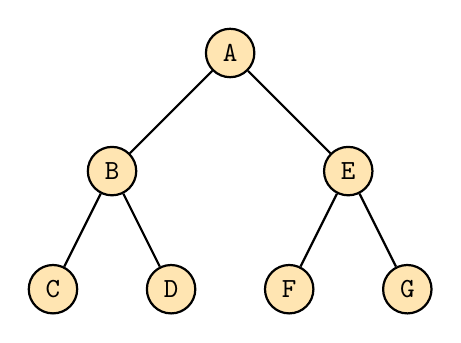
\begin{tikzpicture}[
	level distance=1.5cm,
  level 1/.style={sibling distance=3cm},
  level 2/.style={sibling distance=1.5cm},
	thick,
	font=\ttfamily\bfseries]
  \node[circle,draw,fill=ocra] {A}
    child {node[circle,draw,fill=ocra] {B}
      child {node[circle,draw,fill=ocra] {C}}
      child {node[circle,draw,fill=ocra] {D}}
    }
    child {node[circle,draw,fill=ocra] {E}
    child {node[circle,draw,fill=ocra] {F}}
      child {node[circle,draw,fill=ocra] {G}}
    };
\end{tikzpicture}
}

\end{frame}


%----------------------------------------------------------------------
\begin{frame}{Breadth-First Search}
	
\TwoCols{
\vspace{-12pt}
\begin{Procedure}
\caption[A]{\textsf{bfs}($\Tree\ t$)}
\BlankLine
$\Queue\ Q = \queueconstructor()$\;
$Q.\queueinsert(t)$\;
\While{\NOT\ $Q.\queueempty()$}
{
  $\Tree\ u = Q.\queueremove()$\;
  \alert<2->{\% visita per livelli nodo $u$}\;
  \alert<2->{\PRINT $u$}\;
  $u = u.\treechild()$\;
  \While{$u \neq \Nil$}
  {
    $Q.\queueinsert(u)$\;
    $u = u.\treesibling()$\;
  }
}
\end{Procedure}

}{
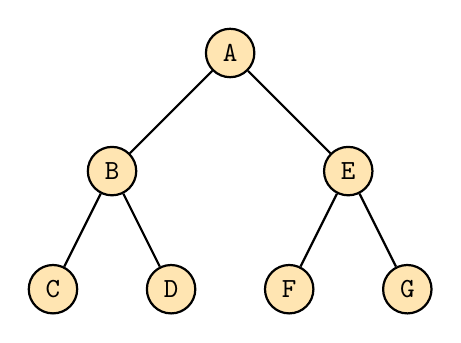
\begin{tikzpicture}[
	level distance=1.5cm,
  level 1/.style={sibling distance=3cm},
  level 2/.style={sibling distance=1.5cm},
	thick,
	font=\ttfamily\bfseries]
  \node[circle,draw,fill=ocra] {A}
    child {node[circle,draw,fill=ocra] {B}
      child {node[circle,draw,fill=ocra] {C}}
      child {node[circle,draw,fill=ocra] {D}}
    }
    child {node[circle,draw,fill=ocra] {E}
    child {node[circle,draw,fill=ocra] {F}}
      child {node[circle,draw,fill=ocra] {G}}
    };

\end{tikzpicture}

\bigskip
\begin{overprint}
\onslide<1|handout:0>
Sequence: \\
Queue: \alert{\texttt{A}}
\onslide<2|handout:0>
Sequence: \alert{\texttt{A}}\\
Queue: \alert{\texttt{B  E}}
\onslide<3|handout:0>
Sequence: \alert{\texttt{A  B}}\\
Queue: \alert{\texttt{E  C  D}}
\onslide<4|handout:0>
Sequence: \alert{\texttt{A  B  E}}\\
Queue: \alert{\texttt{C  D  F  G}}
\onslide<5|handout:0>
Sequence: \alert{\texttt{A  B  E  C}}\\
Queue: \alert{\texttt{D  F  G}}
\onslide<6|handout:0>
Sequence: \alert{\texttt{A  B  E  C  D}}\\
Queue: \alert{\texttt{F  G}}
\onslide<7|handout:0>
Sequence: \alert{\texttt{A  B  E  C  D  F}}\\
Queue: \alert{\texttt{G}}
\onslide<8|handout:1>
Sequence: \alert{\texttt{A  B  E  C  D  F  G}}\\
Queue: 
\end{overprint}
}
\end{frame}

\subsection{Implementazione}

%----------------------------------------------------------------------
\begin{frame}{Memorizzazione}

Esistono diversi modi per memorizzare un albero, più o meno indicati a seconda del numero massimo e medio di figli presenti.

\bigskip
\BIL
\item Realizzazione con vettore dei figli
\item Realizzazione primo figlio, prossimo fratello
\item Realizzazione con vettore dei padri
\EIL

\end{frame}

%----------------------------------------------------------------------
\begin{frame}{Realizzazione con vettore dei figli}

\vspace{-12pt}
\begin{center}
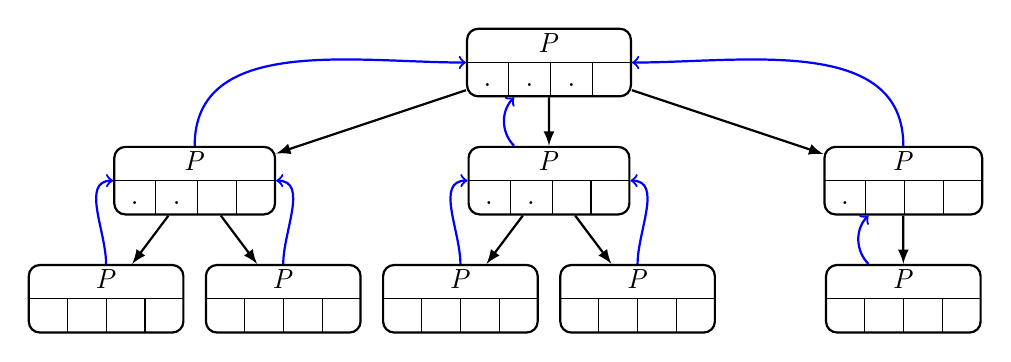
\begin{tikzpicture}[
    level distance=1.5cm,
    level 1/.style={sibling distance=4.5cm},
    level 2/.style={sibling distance=2.25cm},
    edge from parent/.style={draw,-latex},
    thick
]
\node[rounded corners, draw, inner sep=+0pt] (T) {\FD}
  child { node[rounded corners, draw, inner sep=+0pt] (TL) {\FC}
    child { node[rounded corners, draw, inner sep=+0pt] (TLL) {\FA}}
    child { node[rounded corners, draw, inner sep=+0pt] (TLR) {\FA}}
  }
  child { node[rounded corners, draw, inner sep=+0pt] (TC) {\FC}
    child { node[rounded corners, draw, inner sep=+0pt] (TCL) {\FA}}
    child { node[rounded corners, draw, inner sep=+0pt] (TCR) {\FA}}
  }
  child {node[rounded corners, draw, inner sep=+0pt] (TR) {\FB}
    child { node[rounded corners, draw, inner sep=+0pt] (TRL) {\FA}}
  }
;
\draw[->,blue] (TL) to[out=90,in=180] (T);
\draw[->,blue] (TC) to[out=135,in=225] (T);
\draw[->,blue] (TR) to[out=90,in=0] (T);
\draw[->,blue] (TRL) to[out=135,in=225] (TR);
\draw[->,blue] (TLL) to[out=90,in=180] (TL);
\draw[->,blue] (TLR) to[out=90,in=0] (TL);
\draw[->,blue] (TCL) to[out=90,in=180] (TC);
\draw[->,blue] (TCR) to[out=90,in=0] (TC);
\end{tikzpicture}
\end{center}

\begin{myboxtitle}[Campi memorizzati nei nodi]
\BI
\item \alert{$\Parentvar$}: reference al nodo padre
\item \alert{Vettore dei figli}: a seconda del numero di figli, può comportare
una discreta quantità di spazio sprecato
\EI
\end{myboxtitle}
\end{frame}

%----------------------------------------------------------------------
\begin{frame}{Realizzazione basata su Primo figlio, prossimo fratello}

\BB{Implementato come una lista di fratelli}
\begin{center}
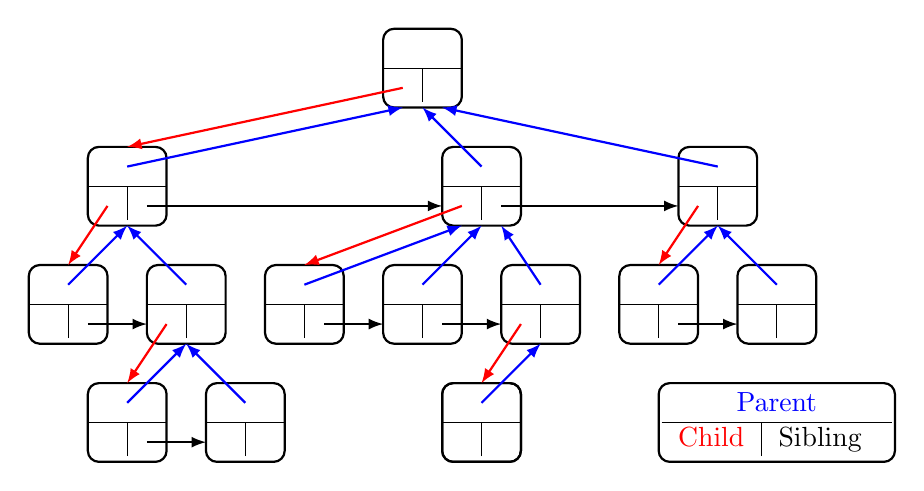
\begin{tikzpicture}[
	level distance=1.5cm,
  level 1/.style={sibling distance=5cm},
  level 2/.style={sibling distance=2.5cm},
	edge from parent/.style={draw,-latex},
	thick
]

\node[rounded corners, draw, inner sep=+0pt,minimum width=1.0cm, minimum height=1.0cm]  at (4.50,3.0) {\FCNB};

\node[rounded corners, draw, inner sep=+0pt,minimum width=1.0cm, minimum height=1.0cm]  at (0.75,1.5) {\FCNB};
\node[rounded corners, draw, inner sep=+0pt,minimum width=1.0cm, minimum height=1.0cm]  at (5.25,1.5) {\FCNB};
\node[rounded corners, draw, inner sep=+0pt,minimum width=1.0cm, minimum height=1.0cm]  at (8.25,1.5) {\FCNB};


\node[rounded corners, draw, inner sep=+0pt,minimum width=1.0cm, minimum height=1.0cm]  at (0.0,0.0) {\FCNB};
\node[rounded corners, draw, inner sep=+0pt,minimum width=1.0cm, minimum height=1.0cm]  at (1.5,0.0) {\FCNB};
\node[rounded corners, draw, inner sep=+0pt,minimum width=1.0cm, minimum height=1.0cm]  at (3.0,0.0) {\FCNB};
\node[rounded corners, draw, inner sep=+0pt,minimum width=1.0cm, minimum height=1.0cm]  at (4.5,0.0) {\FCNB};
\node[rounded corners, draw, inner sep=+0pt,minimum width=1.0cm, minimum height=1.0cm]  at (6.0,0.0) {\FCNB};
\node[rounded corners, draw, inner sep=+0pt,minimum width=1.0cm, minimum height=1.0cm]  at (7.5,0.0) {\FCNB};
\node[rounded corners, draw, inner sep=+0pt,minimum width=1.0cm, minimum height=1.0cm]  at (9.0,0.0) {\FCNB};

\node[rounded corners, draw, inner sep=+0pt,minimum width=1.0cm, minimum height=1.0cm]  at (0.75,-1.5) {\FCNB};
\node[rounded corners, draw, inner sep=+0pt,minimum width=1.0cm, minimum height=1.0cm]  at (2.25,-1.5) {\FCNB};
\node[rounded corners, draw, inner sep=+0pt,minimum width=1.0cm, minimum height=1.0cm]  at (5.25,-1.5) {\FCNB};
\node[rounded corners, draw, inner sep=+0pt,minimum width=1.0cm, minimum height=1.0cm]  at (5.25,-1.5) {\FCNB};


\draw[-latex] (1.00, -1.75) -> (1.75, -1.75);
\draw[-latex] (0.25, -0.25) -> (1.00, -0.25);
\draw[-latex] (3.25, -0.25) -> (4.00, -0.25);
\draw[-latex] (4.75, -0.25) -> (5.50, -0.25);
\draw[-latex] (7.75, -0.25) -> (8.50, -0.25);
\draw[-latex,red] (1.25, -0.25) -> (0.75, -1.00);
\draw[-latex,blue] (0.75, -1.25) -> (1.5, -0.50);
\draw[-latex,blue] (2.25, -1.25) -> (1.5, -0.50);
\draw[-latex,blue] (5.25, -1.25) -> (6, -0.50);
\draw[-latex,red] (5.75, -0.25) -> (5.25, -1.00);

\draw[-latex,red] (0.50, 1.25) -> (0.00, 0.5);
\draw[-latex,blue] (0.00, 0.25) -> (0.75, 1.00);
\draw[-latex,blue] (1.5, 0.25) -> (0.75, 1.00);
\draw[-latex] (1.00, 1.25) -> (4.75, 1.25);

\draw[-latex,red] (5.0, 1.25) -> (3.00, 0.50);
\draw[-latex,blue] (3, 0.25) -> (5.00, 1.00);
\draw[-latex,blue] (4.5, 0.25) -> (5.25, 1.00);
\draw[-latex,blue] (6.0, 0.25) -> (5.50, 1.00);
\draw[-latex] (5.50, 1.25) -> (7.75, 1.25);


\draw[-latex,red] (8.00, 1.25) -> (7.5, 0.50);
\draw[-latex,blue] (7.5, 0.25) -> (8.25, 1.00);
\draw[-latex,blue] (9.0, 0.25) -> (8.25, 1.00);

\draw[-latex,red] (4.25, 2.75) -> (0.75, 2.00);
\draw[-latex,blue] (0.75, 1.75) -> (4.25, 2.50);
\draw[-latex,blue] (5.25, 1.75) -> (4.50, 2.50);
\draw[-latex,blue] (8.25, 1.75) -> (4.75, 2.50);

\node[rounded corners, draw, inner sep=+0pt,minimum width=3.0cm, minimum height=1.0cm]  at (9,-1.5) {
  \begin{tabular}{c|c}
    \multicolumn{2}{c}{\textcolor{blue}{Parent}} \\\hline
     \textcolor{red}{Child} & Sibling \, 
  \end{tabular}
};

\end{tikzpicture}
\end{center}
	
	
\end{frame}

%----------------------------------------------------------------------
\begin{frame}[shrink=25]{Implementazione}
\vspace{-12pt}
\begin{Procedure}
\caption[A]{\Tree}
\BlankLine

\Tree \Parentvar\REMR{Reference al padre}
\Tree \Childvar\REMR{Reference al primo figlio}
\Tree \Siblingvar\REMR{Reference al prossimo fratello}
\Item \Valuevar\REMR{Valore memorizzato nel nodo}
\BlankLine

\PROCEDURE{\treeconstructor(\Item $v$)\REMF{Crea un nuovo nodo}}
{
  $\Tree\ t = \NEW\ \Tree$\;
  $t.\Valuevar = v$\;
  $t.\Parentvar = t.\Childvar = t.\Siblingvar = \Nil$\;
  \Return $t$\;
}
\BlankLine

\PROCEDURE{\insertchild(\Tree $t$)}
{
$t.\Parentvar = \textbf{self}$\;
$t.\Siblingvar = \Childvar$\REMR{Inserisce $t$ prima dell'attuale primo figlio}
$\Childvar = t$\;
}
\BlankLine

\PROCEDURE{\insertsibling(\Tree $t$)}
{
$t.\Parentvar = \Parentvar$\;
$t.\Siblingvar = \Siblingvar$\REMR{Inserisce $t$ prima dell'attuale prossimo fratello}
$\Siblingvar = t$\;
}
\BlankLine
\end{Procedure}

\end{frame}

%----------------------------------------------------------------------
\begin{frame}[shrink=25]{Implementazione}
\vspace{-12pt}
\begin{Procedure}
\caption[A]{\Tree}

\PROCEDURE{\deletechild()}
{
  $\Tree\ \mathit{newChild} = \Childvar.\treesibling()$\;
  $\treedelete(\Childvar)$\;
  $\Childvar = \mathit{newChild}$\;
}
\BlankLine

\PROCEDURE{\deletesibling()}
{
  $\Tree\ \mathit{newSibling} = \Siblingvar.\treesibling()$\;
  $\treedelete(\Siblingvar)$\;
  $\Siblingvar = \mathit{newSibling}$\;
}
\BlankLine

\PROCEDURE{\treedelete(\Tree $t$)}
{
  $\Tree\ u = t.\treechild()$\;
  \While{$u \neq \Nil$}
  {
    $\Tree\ \textit{next} = u.\treesibling()$\;
    $\treedelete(u)$\;
    $u = \textit{next}$\;
  }
  \DELETE $t$\;
}

\end{Procedure}

\end{frame}

%----------------------------------------------------------------------
\begin{frame}{Realizzazione con vettore dei padri}

L'albero è rappresentato da un vettore i cui elementi contengono il valore associato al nodo e l'indice della posizione del padre nel vettore.

\begin{multicols}{2}
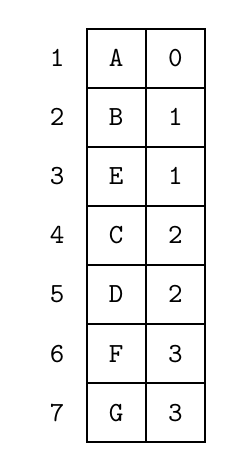
\begin{tikzpicture}[
    thick,
	font=\ttfamily\bfseries
    ]
\node[rectangle, draw, inner sep=+0pt,minimum width=0.75cm, minimum height=0.75cm]  at (0.00,-0.00) {A};
\node[rectangle, draw, inner sep=+0pt,minimum width=0.75cm, minimum height=0.75cm]   at (0.75,-0.00) {0};
\node[rectangle, draw, inner sep=+0pt,minimum width=0.75cm, minimum height=0.75cm]  at (0.00,-0.75) {B};
\node[rectangle, draw, inner sep=+0pt,minimum width=0.75cm, minimum height=0.75cm]   at (0.75,-0.75) {1};
\node[rectangle, draw, inner sep=+0pt,minimum width=0.75cm, minimum height=0.75cm]  at (0.00,-1.50) {E};
\node[rectangle, draw, inner sep=+0pt,minimum width=0.75cm, minimum height=0.75cm]   at (0.75,-1.50) {1};
\node[rectangle, draw, inner sep=+0pt,minimum width=0.75cm, minimum height=0.75cm]  at (0.00,-2.25) {C};
\node[rectangle, draw, inner sep=+0pt,minimum width=0.75cm, minimum height=0.75cm]   at (0.75,-2.25) {2};
\node[rectangle, draw, inner sep=+0pt,minimum width=0.75cm, minimum height=0.75cm]  at (0.00,-3.00) {D};
\node[rectangle, draw, inner sep=+0pt,minimum width=0.75cm, minimum height=0.75cm]   at (0.75,-3.00) {2};
\node[rectangle, draw, inner sep=+0pt,minimum width=0.75cm, minimum height=0.75cm]  at (0.00,-3.75) {F};
\node[rectangle, draw, inner sep=+0pt,minimum width=0.75cm, minimum height=0.75cm]   at (0.75,-3.75) {3};
\node[rectangle, draw, inner sep=+0pt,minimum width=0.75cm, minimum height=0.75cm]  at (0.00,-4.50) {G};
\node[rectangle, draw, inner sep=+0pt,minimum width=0.75cm, minimum height=0.75cm]   at (0.75,-4.50) {3};

\node[minimum width=0.75cm, minimum height=0.75cm]   at (-0.75,-0.00) {1};
\node[minimum width=0.75cm, minimum height=0.75cm]   at (-0.75,-0.75) {2};
\node[minimum width=0.75cm, minimum height=0.75cm]   at (-0.75,-1.50) {3};
\node[minimum width=0.75cm, minimum height=0.75cm]   at (-0.75,-2.25) {4};
\node[minimum width=0.75cm, minimum height=0.75cm]   at (-0.75,-3.00) {5};
\node[minimum width=0.75cm, minimum height=0.75cm]   at (-0.75,-3.75) {6};
\node[minimum width=0.75cm, minimum height=0.75cm]   at (-0.75,-4.50) {7};



\end{tikzpicture}

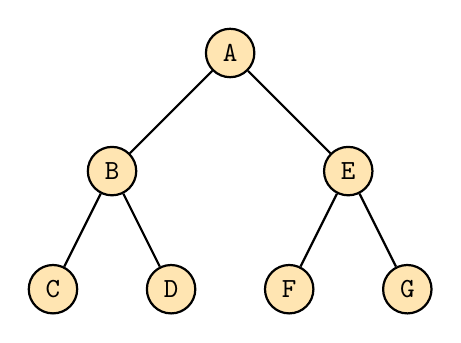
\begin{tikzpicture}[
	level distance=1.5cm,
  level 1/.style={sibling distance=3cm},
  level 2/.style={sibling distance=1.5cm},
	thick,
	font=\ttfamily\bfseries]
  \node[circle,draw,fill=ocra] {A}
    child {node[circle,draw,fill=ocra] {B}
      child {node[circle,draw,fill=ocra] {C}}
      child {node[circle,draw,fill=ocra] {D}}
    }
    child {node[circle,draw,fill=ocra] {E}
    child {node[circle,draw,fill=ocra] {F}}
      child {node[circle,draw,fill=ocra] {G}}
    };

\end{tikzpicture}
\end{multicols}


\end{frame}

%----------------------------------------------------------------------
\begin{OnlySlides}{DFS (\url{https://xkcd.com/})}

\IG{0.7}{dfs.png}

\end{OnlySlides}


\end{document}
%%%%%%%%%%%%%%%%%%%%%%%%%%%%%%%%%%%%%%%%%%%%%%%%%%%%%%%%%%%%%%%%%%%%%%%%%%

